\chapter{Análisis y evaluación de \\herramientas de textos médicos}

En este capítulo discutiremos cómo hemos llevado a cabo la evaluación de las herramientas disponibles en el estado del arte para la extracción de información en texto no estructurado de carácter médico.

Para ello se ha creado una web app disponible de forma muy accesible para que sea fácil ver el poder combinado de todas estas herramientas. Dicha herramienta se denomina \href{https://share.streamlit.io/jesi-rgb/medical-text-analysis/src/streamlit_gen_test.py}{MEDGEN}.

\section{Estado del arte: análisis de textos médicos}

Para el análisis y minería de texto no estructurado una de las técnicas más útiles es el \textbf{Named Entity Recognition (NER) Tagging}, es decir, el etiquetado de entidades. La idea es, dado un cuerpo de texto, extraer aquellas entidades que tengan un significado propio o relevante por sí mismas. En nuestro contexto, esto corresponde, por ejemplo, a nombres de enfermedades, partes del cuerpo, medicamentos, entre otras. Un NER Tagger entrenado sería capaz de detectar dichas entidades en el texto y devolver una lista de las mismas, automatizando la extracción de información.

La librería SciSpacy \cite{neumann-etal-2019-scispacy} nos provee con una selección de NER Taggers preentrenados en diferentes corpus de caracter biomédico y los hace disponibles mediante la famosa librería Spacy \cite{spacy}, que se ha convertido en el estándar de la industria para el análisis del lenguaje natural.

Estos son los taggers que utilizaremos en nuestra aplicación, aunque resulta sencillo incluir algún otro más que pudiera ser de interés.

\begin{itemize}
	\item \textbf{Med7} \cite{med7}: El Med7 es un NER entrenado en datos clínicos capaz de detectar 7 entidades diferentes: nombres de medicamentos (Aspirina, Advil), vía de administración del medicamento (oral, intravenosa, respiratoria), frecuencia (cada 8 horas), dosis (mg o ml), cantidad (número de pastillas), formato (pastilla, polvos, etc), y tiempo total de medicación (semanas, meses). 
	\item \textbf{BC5CDR} \cite{bc5cdr}: Este tagger recibe su nombre del corpus en el que fue entrenado. Dicho corpus consta de 1500 artículos \textit{PubMed} con 4409 sustancias químicas etiquetadas, 5818 enfermedades y 3116 interacciones enfermedad-medicamento.
	\item \textbf{BIONLP13CG} \cite{BIONLP13CG}: De igual forma, este tagger recibe su nombre del corpus que lo origina. Este tagger se especializa más en términos genéticos, cánceres, órganos y compuestos químicos como aminoácidos o proteínas, ligeramente mejor adecuado para prescripciones quirúrgicas.
\end{itemize}

\begin{figure}[h]
	\centering
	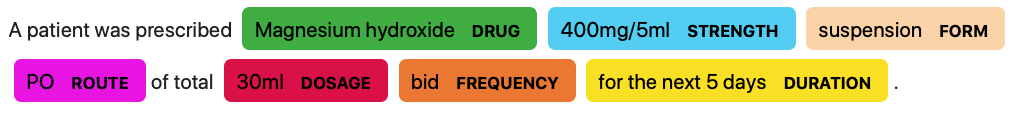
\includegraphics[width=.9\textwidth]{media/med7_example.png}
	\caption{Ejemplo del Med7 en acción. Vemos cómo las entidades se han reconocido en diferentes colores, haciendo la extracción de información mucho más eficiente. bid viene del latin \textit{bis in die}, que se traduce por dos veces al día. PO viene de \textit{Per os}, vía oral. \textit{Suspension} hace referencia a una disolución en agua.}
	\label{fig:med7}
\end{figure}

En la Figura \ref{fig:med7} vemos un ejemplo de cómo una de estas herramientas puede ayudar al análisis del texto, destacando con diferentes colores las entidades encontradas. Esto es, sin embargo, solo una aplicación de demostración. El verdadero poder reside en que dichas entidades están internamente representadas en forma de diccionario, asociando cada término encontrado en el texto con la entidad correspondiente. 

Estos diccionarios pueden anexarse y guardarse en la base de datos correspondiente, haciendo su búsqueda y análisis muchísimo más rápidos, además de habilitando comparativas que no serían posibles de otra forma.


\section{Despliegue de MEDGEN}

Para hacer accesible todo el trabajo que se ha acometido, se ha elaborado una aplicación que permite hacer uso de todas las técnicas y herramientas discutidas a lo largo del documento. 

El framework utilizado ha sido \href{https://streamlit.io}{Streamlit}. Streamlit es un framework para Python diseñado para el prototipado ágil de aplicaciones web. Los creadores idearon esta herramienta para disminuir el esfuerzo que hay que acometer a la hora de desplegar una aplicación basada en inteligencia artificial, es decir, una aplicación que consta de sistemas de inferencia o similares, sistemas que no se encuentran en aplicaciones web usuales. 

De esta forma, es muy accesible y sencillo diseñar una aplicación en Python, donde se puede integrar cualquier sistema de IA en desarrollo y habilitar un espacio para que personas ajenas al desarrollo experimenten de primera mano cómo funciona, ofreciendo la oportunidad de crear casos de uso reales.

La aplicación permite generar comentarios utilizando el modelo generativo, y permite analizar dichos comentarios, así como importar desde distintas fuentes. La aplicación efectúa un pequeño análisis del texto y utiliza el tagger que el usuario seleccione.


Como vemos en las Figuras \ref{fig:app-demo} y \ref{fig:analysis-comment}, podemos efectuar nuestro análisis de diferentes formas.

Podemos, en caso de no disponer de un conjunto de datos, generar comentarios usando nuestro modelo generativo. Una vez generados, podemos analizarlos con el NER Tagger que deseemos. Aquí el desarrollador estaría desarrollando el suyo propio y podría integrarlo al sistema fácilmente para testearlo de forma apropiada. 

El análisis nos ofrece una versión etiquetada del texto original, así como unas estadísticas del comentario en concreto.

Además de ello, podemos importar nuestros propios comentarios desde un archivo o copiarlos y pegarlos en el campo de texto, con tal de maximizar la comodidad de uso de la aplicación.

\begin{figure}[h]
	\centering
	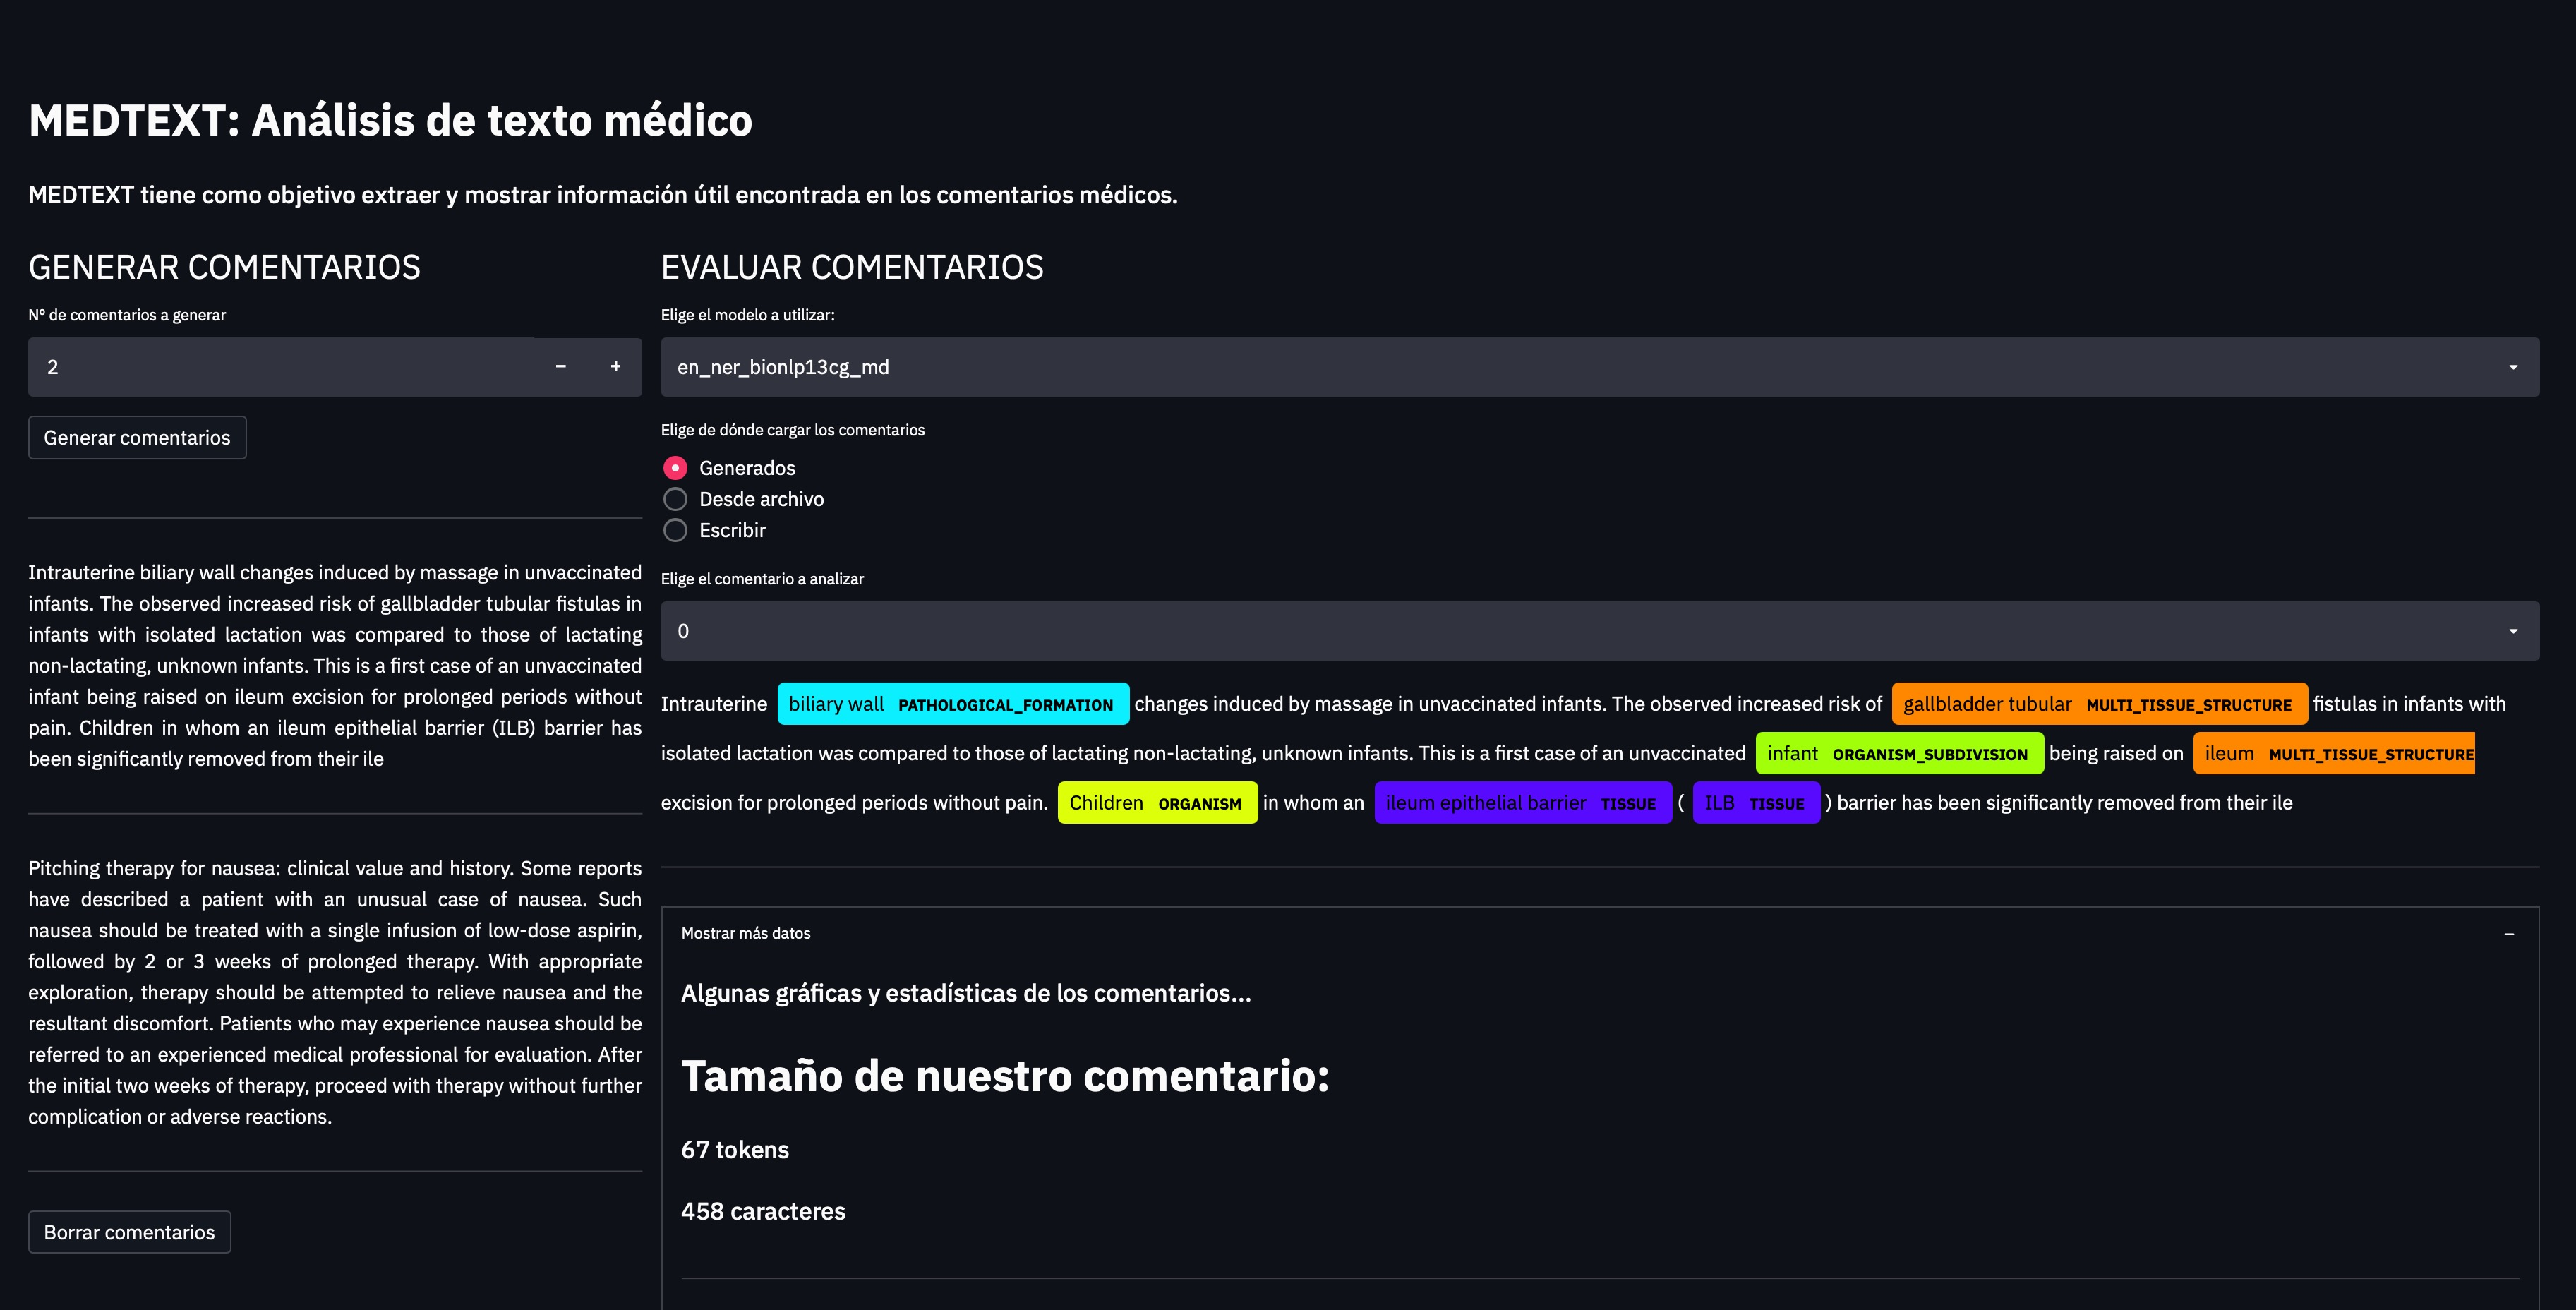
\includegraphics[width=.9\textwidth]{media/app_demo.jpeg}
	\caption{Captura de pantalla de la aplicación elaborada. A la izquierda podemos generar comentarios y a la derecha, analizarlos.}
	\label{fig:app-demo}
\end{figure}


\begin{figure}[t]
	\centering
	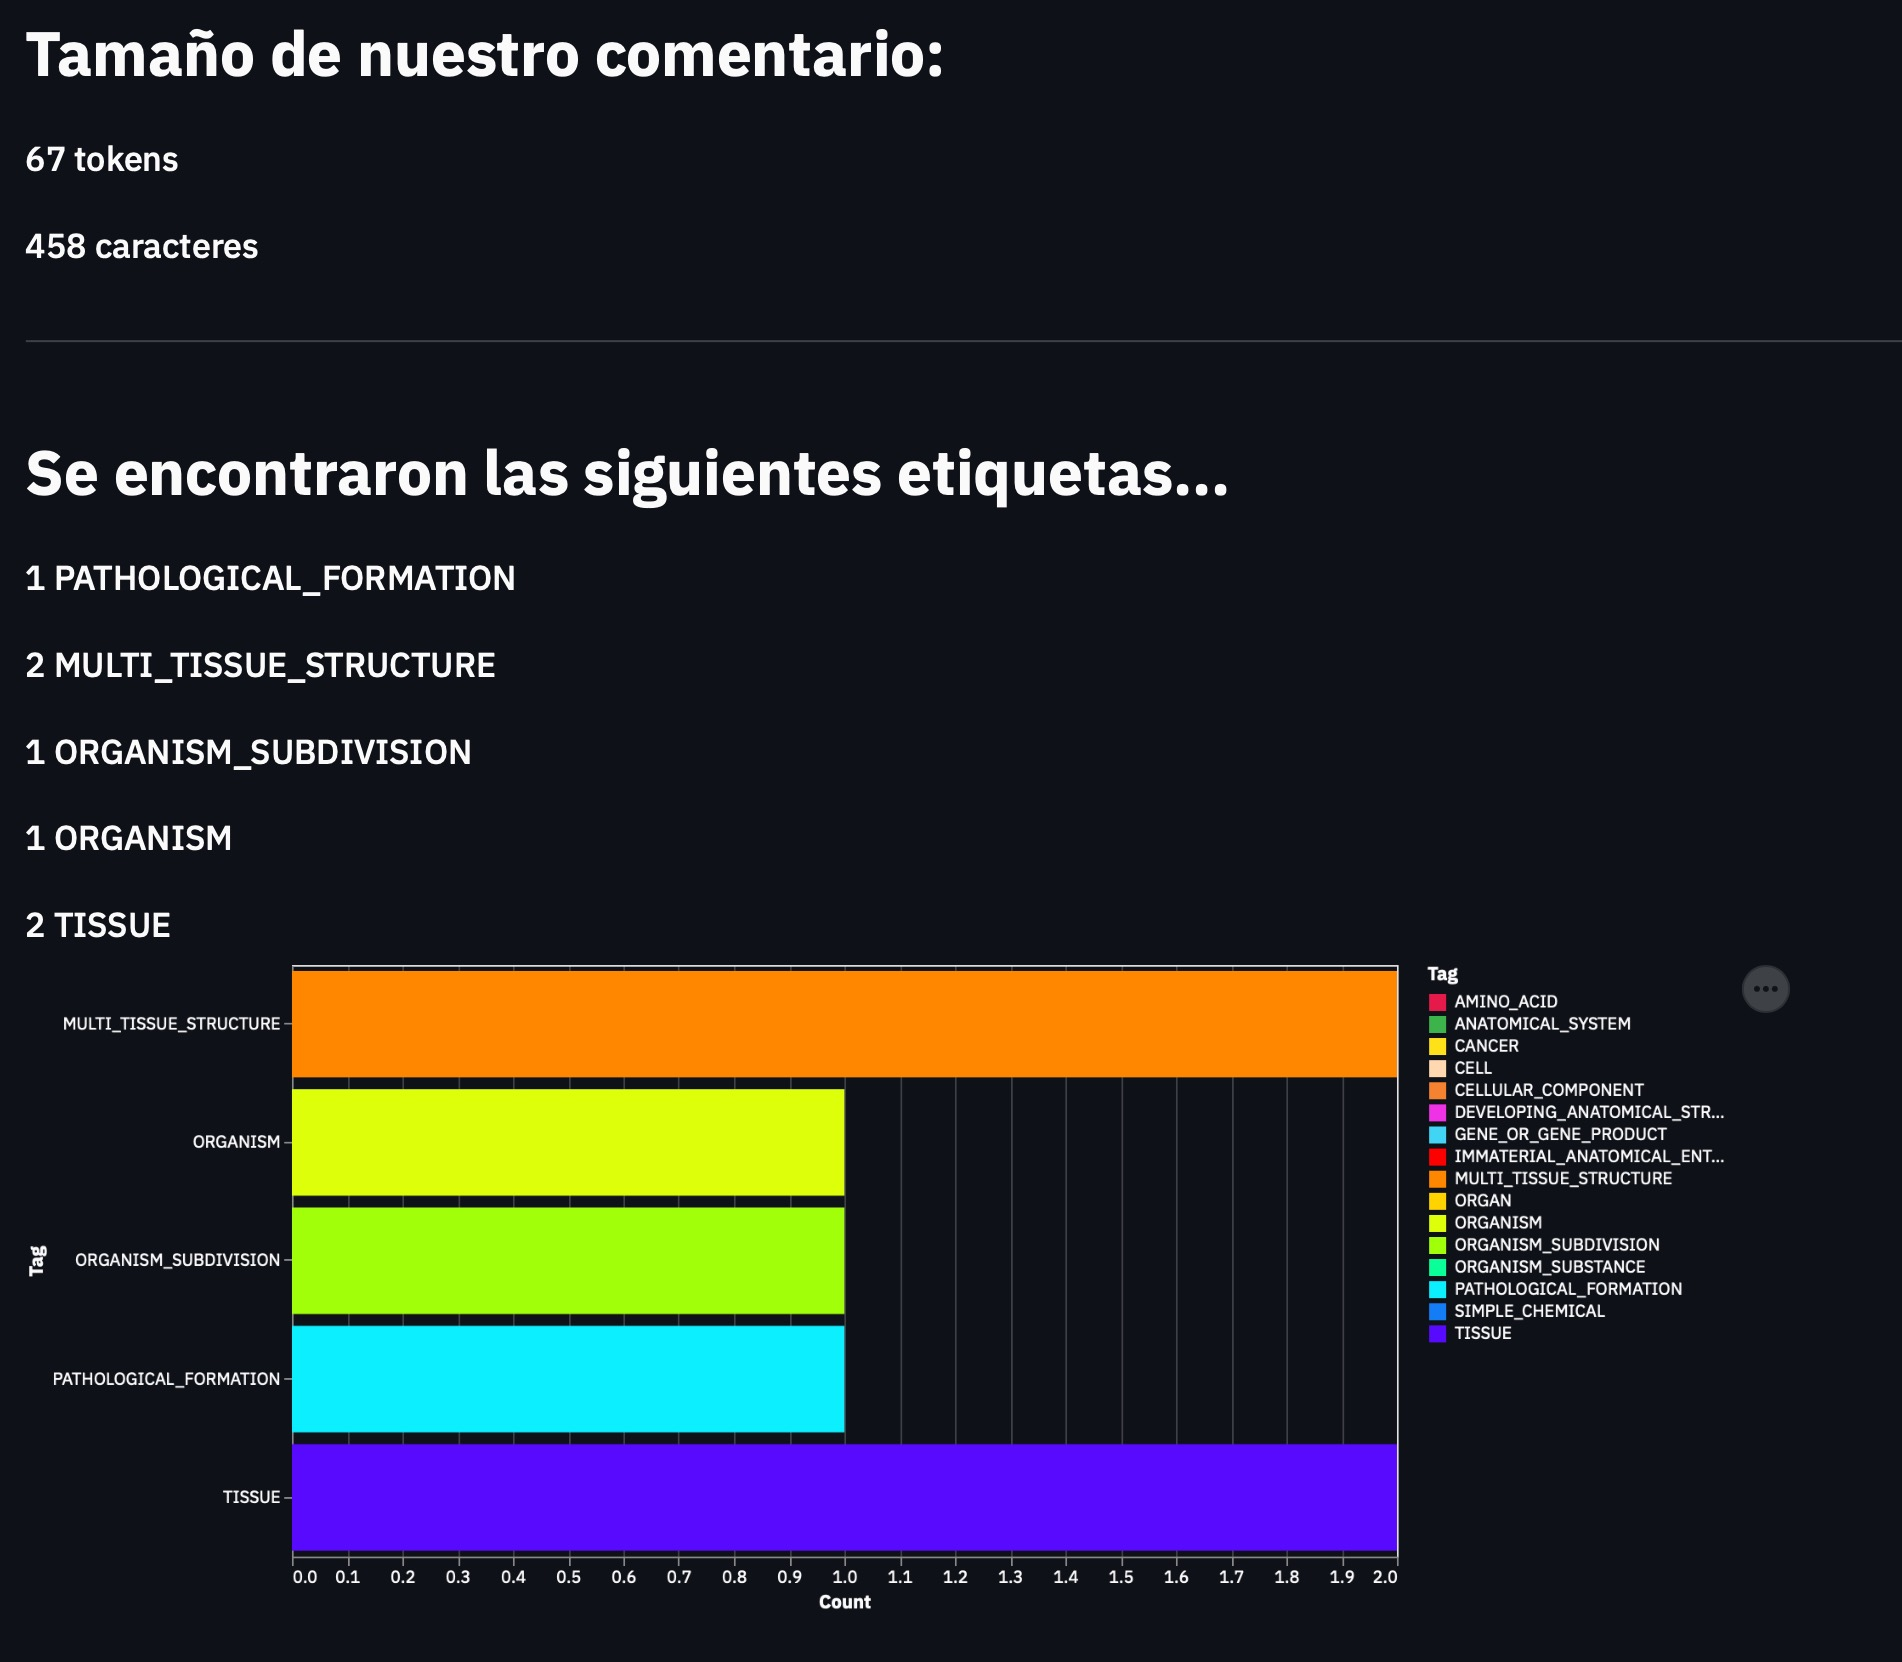
\includegraphics[width=.62\textwidth]{media/analysis_comment.jpeg}
	\caption{Captura de pantalla del análisis que ofrece la aplicación acerca de un determinado comentario.}
	\label{fig:analysis-comment}
\end{figure}



\section{Instalación y modo de uso}
La aplicación puede compilarse desde el código fuente siguiendo el \href{https://github.com/jesi-rgb/medical-text-analysis}{enlace al repositorio}, descargándolo y ejecutando los siguientes comandos:

\jesitt{git clone https://github.com/jesi-rgb/medical-text-analysis}

Activamos el entorno que más nos guste, ya sea de python o conda.

\jesitt{cd medical-text-analysis}

\jesitt{pip install -r requirements.txt}

Una vez finalizado, 

\jesitt{streamlit run src/streamlit\_gen\_test.py}

se nos abrirá una ventana en el navegador y la aplicación estará lista para funcionar.

La primera ejecución tarda un poco más, ya que ha de descargar el modelo de Internet y cargarlo en memoria. Tras eso, los modelos se guardan en caché y la ejecución es mucho más rápida.
